\section{Red Blood Cells Composition} \label{Sect.Blood}


\noindent There are around 25 trillion \ac{rbc} within the human body \cite{Cimen2008}. A \acf{rbc} is scientifically known as an erythrocyte, the word has Greek origins with erythros meaning red and -cyte meaning cell. A \ac{rbc}'s principle purpose is to deliver \ac{o2} to the body tissue via blood flow in the circulatory system. In humans, \ac{rbc} take up oxygen in the lungs and release it into tissues while squeezing through the body's capillaries. The dynamic shape of the \ac{rbc} is critical to the transportation and release of \ac{o2} within the blood stream and is if great importance to understand.

A typical healthy \ac{rbc} comprises of only 2 main parts: the cytoplasm and the cell membrane. The cytoplasm of erythrocytes is rich in hemoglobin. Hemoglobin is an iron-containing biomolecule that binds to oxygen and is responsible for the distinct red colour \cite{Shape2010}. The cell membrane is composed of proteins and lipids that control the inflow and outflow of the cell along with the physical properties essential for deformability and structural stability. Unlike almost all other cells in the human body \ac{rbc}s `anucleate' when mature, this means that they lack a cell nucleus \cite{redblood2009}. In addition, \ac{rbc}s also lack other intracellular organelles. These deficits enhances the ability for a \ac{rbc} to deform when traversing the circulatory system and specifically the capillary network.


A healthy, mature  \ac{rbc} is shaped as an oval biconcave disk. They are often viewed as `sacks of hemoglobin, with a plasma membrane'. Approximately 2.4 million new erythrocytes are produced per second in human adults \cite{Minasyan2014} and have a life of around 100–120 days \cite{Minasyan2014, Kim1979} before being recycled within the body. Each circulation takes about 60 seconds in which an erythrocyte will intake \ac{o2} in the lungs, be pumped by the heart, traverse the circulatory system to the desired location, enter the capillary network in which the \ac{rbc} will deform releasing the \ac{o2}, then, finally, return to the lungs via the heart \cite{Minasyan2014, Kim1979}. 

A typical human \ac{rbc} has a disk diameter of approximately $6.2–8.2 \mu m$ \cite{Shape2010} and a thickness at the thickest point of 2–2.5$\mu m$ with a minimum thickness in the centre of 0.8–1$\mu m$ \cite{Shape2010}. These cells have an average volume of about $90 f$L ($1f$L$ = 10^{-15}$L) with a surface of about 136 $\mu m^2$ \cite{Shape2010}. A \ac{rbc} can swell up to a sphere shape containing $150 f$L, without membrane distension \cite{Minasyan2014}.


\subsection{Membrane composition}
\noindent \ac{rbc} membrane plays a key role in the cells ability to deform, flex, adhere to other cells and to interface with immune cells. The abilities of each are dependent on the specific membrane composition. A \ac{rbc} membrane is composed of 3 layers. The glycocalyx on the exterior, which is rich in carbohydrates, the lipid bilayer which contains many transmembrane proteins alongside its lipidic main constituents and the membrane skeleton, a structural network of proteins located on the inner surface of the lipid bilayer \cite{redblood2009, Shape2010} (Figure \ref{fig.rbc.wall}). 

\begin{figure}[H]
	\centering
	
	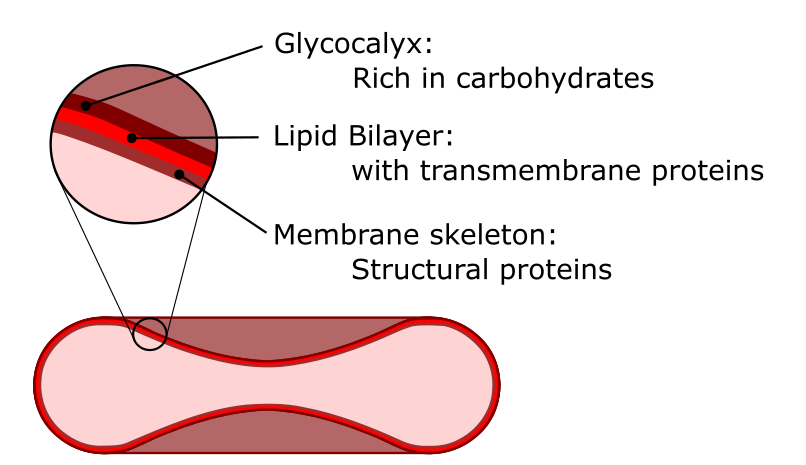
\includegraphics[width=0.5\linewidth]{fig/rbc}
	
	\caption{Pictorial of a cross-section of a \ac{rbc} with zoom on the membrane comprising of three layers. Image created by M. Goodman  }
	\label{fig.rbc.wall}
\end{figure}

\noindent The outer monolayer is comprised of Phosphatidylcholine (PC) and Sphingomyelin (SM) compared to the inner monolayer which is comprised of Phosphatidylethanolamine (PE) small amounts of Phosphoinositol (PI) and Phosphatidylserine (PS) \cite{Quinn2002}. Note, in this research only, all the layers of the cell membrane will be referred to as the cell wall.


\subsubsection*{Membrane lipids}
\noindent The membrane is similar to other cells in the human body and is not unique to the \ac{rbc}. The \ac{rbc} membrane comprises a typical lipid bilayer, composed of cholesterol and phospholipids in equal proportions by weight \cite{redblood2009} (Figure \ref{fig.rbc.lipid}). The composition of the lipid bilayer defines many physical properties including the membrane permeability and fluidity. The lipids in the bilayer also help regulate the activity of many membrane proteins.

\begin{figure}[H]
	\centering
	
	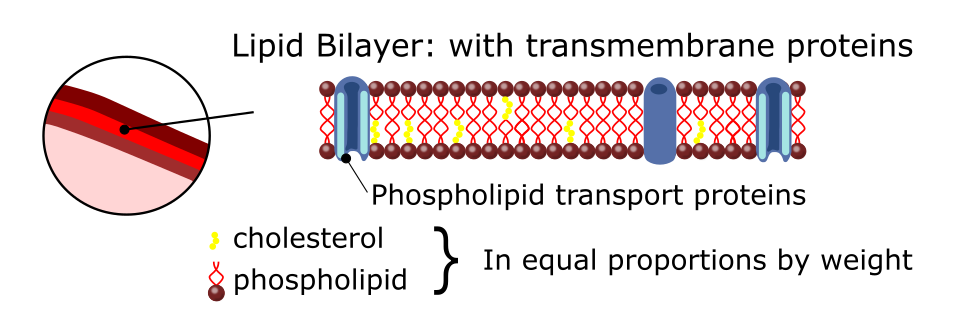
\includegraphics[width=0.8\linewidth]{fig/Lipidbylayer}
	
	\caption{Pictorial of \ac{rbc} cell membrane, lipid bilayer detail including cholesterol, phospholipids and transport proteins. Image created by M. Goodman }
	\label{fig.rbc.lipid}
\end{figure}


\subsubsection*{Membrane proteins}
\noindent The proteins of the membrane skeleton, responsible for the deformability, flexibility and durability, enable a \ac{rbc} to squeeze through capillaries less than half the diameter of the \ac{rbc} and recovering the discoid shape as soon as these cells stop receiving compressive forces. There are currently more than 50 different types of membrane proteins, with a possible of a few hundred to a million copies per \ac{rbc} \cite{redblood2009}. Approximately 25 of these membrane proteins carry the various blood group antigens, such as the A, B, Rh antigens, etc \cite{redblood2009}. The membrane proteins perform a wide diversity of functions such as transporting ions and molecules across the red cell membrane, adhesion, interaction with other cells (endothelial cells), signaling receptor and many others \cite{redblood2009}. Problems with the proteins in these membranes are associated with multiple disorders, such as hereditary spherocytosis, hereditary elliptocytosis, hereditary stomatocytosis, and paroxysmal nocturnal hemoglobinuria.

\subsection{Hereditary Spherocytosis (HS)} \label{Sect.HS}
\noindent \ac{hs}  is a congenital \ac{rbc} membrane disorder characterized by spherical \ac{rbc}s that have reduced diameter (microspherocytosis) and are intensely hemoglobinized (carrying more hemoglobin than normal) \cite{Shape2010}. \ac{hs} is the most common hereditary \ac{rbc} membrane disorder found and affects approximately 1 in 2,000 individuals of northern European ancestry \cite{redblood2009}. \ac{hs} is caused by heterogeneous defects in proteins that vertically connect the membrane skeleton to the lipid bilayer\cite{redblood2009} (see Figure \ref{fig.rbc.wall}). Interactions dependent on vertical connection are thought to play a role in the mechanical stability of the \ac{rbc} membrane \cite{Shape2010}. \ac{hs} causes a loss of spectrin density resulting in a greater maximum stretch that a membrane can undergo beyond which it is unable to recover to its original shape. Spectrin network connectivity can be as low as 3.3 spectrin per actin for cases of \ac{hs} compared to ~5 spectrin molecules bound to each actin filament \cite{redblood2009,Shape2010,Minasyan2014}. The process of \ac{rbc} surface area loss happens more rapidly than volume loss, which results in the formation of spherical \ac{rbc}s with decreased deformability. In healthy patients \ac{rbc}s with decreased membrane surface area are unable to effectively traverse the spleen and are subsequently removed from circulation by the spleen \cite{Shape2010}. The changes seen in \ac{hs} \ac{rbc}s are also seen in non-hereditary spherocytosis, however, typically less severe.

For the purposes of this research, the \ac{rbc} modelling approximations will be modelled after a spherical \ac{rbc} with any properties not obtainable from a \ac{hs} \ac{rbc} will be approximated as a healthy \ac{rbc}.


\subsection{Cell Properties}
\noindent There are many measurable and derived properties of a cell from experiments and accepted modelling techniques. Here a short overview of related properties is given. Table \ref{table.rbc.prop} contains the physical properties of a healthy blood cell. These properties were found by \citet{ademiloye2016} using approximation methods and computer simulations to give the best results. Thus, these properties are dependent upon on two parameters; $k_a$ and $k_v$ the area and volume constraint respectively. These values were also compared to literature and found to reasonable approximations. 
\\
\noindent
\begin{table} [H]
	\begin{center}
		\caption{ Physical properties of a healthy \ac{rbc} membrane where the area and volume constraints, $k_a$ and $k_v$ respectively are equal.   \ }
		\label{table.rbc.prop}
		\begin{tabularx} {0.95\textwidth}{L{7cm} R{1.5cm} R{1.5cm} R{1.5cm} R{1.5cm} }
			\hline
			\multicolumn{1}{l}{\textbf{Elastic Properties}} & \multicolumn{4}{c}{\textbf{$k_a = k_v = \xi$}}  \\ 
			\multicolumn{1}{l}{\textbf{(Symbol [units])}} & \textbf{$0$} & \textbf{$ 100$} 	& \textbf{$ 150$} 	& \textbf{$300$}  \\  
			\hline
			\multicolumn{1}{l}{Young's Modulus (E) $[\mu Nm^{-1}]$}			  & 22.13 				& 21.42 			& 19.31 		 	& 17.31 \\
			\multicolumn{1}{l}{Poisson's Ratio ($v$) }						  &	0.33 				& 0.46 				& 0.45 			& 0.44 \\
			\multicolumn{1}{l}{Shear Modulus ($\mu _h$) $[\mu Nm^{-1}]$}	 &		7.98 			&		7.49 		& 6.70 	&				6.00 \\
			\multicolumn{1}{l}{Area Compression Modulus ($K) [\mu Nm^{-1}]$} &	15.96 				&		20.14 		& 17.65 &				15.55 \\
			\multicolumn{1}{l}{Bending Modulus (B) $[\times 10^{-14}$ J]}	 &	 6.26				&		 5.87 		& 5.25 	&				4.71 \\
			\hline
			
		\end{tabularx}
	\end{center}
\end{table}

\noindent Arterial blood pressure is found at the maximum state (systole) to be 13-18 kPa and in the minimum state (diastole) to be 8-12 kPa. Note the common unit for arterial blood pressure is millimetres of mercury. 

Finally, average dimensions of a \ac{rbc} need to be considered. A healthy \ac{rbc}s has a diameter of 6.2 to 7.2 $\mu m$ \cite{redblood2009,ademiloye2016,Shape2010,Kim1979,HHSPublic2016} with a \acf{hs} \ac{rbc} being less than this. The cell wall thickness is of the order 100 A \cite{Fung1968} (where 1 Angstrom (A) is a unit of length equal to $10^{-10} m$)  i.e. $100 \times 10^{-10} m = 10^{-8} m = 10 nm$ or the ratio of cytosol radius to wall is approximately 360:1. 


